\chapter*{Εκτενής Περίληψη}
\addcontentsline{toc}{chapter}{Εκτενής Περίληψη}

\begin{greek}

Συστήματα ρομποτικής χρησιμοποιούνται εκτενώς στο CERN, καθώς με αυτόν τον τρόπο αυξάνεται η αξιοπιστία και η ασφάλεια των επιταχυντών, αφού μπορούν να πραγματοποιούνται πιο άμεσες επεμβάσεις και έρευνες για πιθανά προβλήματα που προκύπτουν, καθώς και χειρισμός αδιευκρίνιστων αντικειμένων. Επιπλέον, επιτυγχάνεται μείωση της έκθεσης του ανθρώπινου δυναμικού σε συνθήκες που ενέχουν κινδύνους και πηγάζουν από το αντίξοο περιβάλλον των επιταχυντών, όπως υψηλά επίπεδα ακτινοβολίας, παρουσία ραδιενεργών πηγών ή έλλειψη οξυγόνου στις υπόγειες εγκαταστάσεις.

Καθώς οι προσπάθειες σχεδιασμού του Μελλοντικού Κυκλικού Επιταχυντή~(FCC), ενός νέου επιταχυντή με περίμετρο περίπου 100~χιλιομέτρων, εντείνονται, εξετάζονται ρομποτικά συστήματα τα οποία θα εγκατασταθούν εντός της σήραγγας, ώστε να διασφαλίσουν τη μέγιστη δυνατή διαθεσιμότητα λειτουργίας του. Επομένως, ένα από τα πρώιμα στάδια προς αυτή την κατεύθυνση, και ο στόχος της παρούσας εργασίας, είναι ο σχεδιασμός του συστήματος ελέγχου των κινητήρων, τόσο σε επίπεδο υλικού όσο και λογισμικού, με βασικό γνώμονα και πρόκληση την προϋπόθεση να είναι ανθεκτικό κατά τη λειτουργία του σε περιβάλλοντα πολύ υψηλής ακτινοβολίας.

Το πρώτο στάδιο είναι η επιλογή του τύπου ηλεκτρικού κινητήρα που θα χρησιμοποιηθεί για τις δοκιμές. Με τη λογική ότι η εφαρμογή αφορά ρομποτικά συστήματα και, πιο συγκεκριμένα, ρομποτικούς βραχίονες, και θα απαιτεί όσο το δυνατόν χαμηλότερη συντήρηση και υψηλότερη ενεργειακή αυτονομία, επιλέχθηκε ένας κινητήρας τύπου Brushless DC~(BLDC). Το βασικό του πλεονέκτημα είναι ότι η κατασκευαστική του λογική δεν βασίζεται σε μηχανική αλλά σε ηλεκτρονική μεταγωγή. Με την κατάλληλη διαμόρφωση των ρευμάτων του στάτορα δημιουργείται ένα περιστρεφόμενο μαγνητικό πεδίο, το οποίο, σε αλληλεπίδραση με το μόνιμο πεδίο των μαγνητών του ρότορα, παράγει ροπή. Επιπλέον, υπάρχουν τεχνικές οδήγησης που επιτυγχάνουν πολύ υψηλό επίπεδο απόδοσης και ακρίβειας. Η τεχνική Field-Oriented Control~(FOC) που επιλέχθηκε επιτρέπει την αποτελεσματική παραγωγή ροπής, καθώς και μεγάλη ακρίβεια στον έλεγχο ταχύτητας και θέσης, ενώ παράλληλα είναι εφαρμόσιμη και σε άλλους τύπους κινητήρων, όπως οι βηματικοί κινητήρες και οι ασύγχρονοι κινητήρες εναλλασσόμενου ρεύματος~(AC Induction Machines, ACIM). Επομένως, με αυτή τη λύση, η στόχευση είναι η ανάπτυξη και αξιολόγηση ενός όσο το δυνατόν πιο γενικού και αντιπροσωπευτικού συστήματος οδήγησης κινητήρα, το οποίο θα μπορεί να ενσωματωθεί σε μεγαλύτερα συστήματα.

Το πρώτο στάδιο της ανάπτυξης περιλαμβάνει τον καθορισμό των απαραίτητων εξαρτημάτων, ο οποίος προκύπτει σε μεγάλο βαθμό από τον αλγόριθμο οδήγησης. Καταρχάς, το θεμελιώδες στοιχείο είναι η δημιουργία ενός τριφασικού αντιστροφέα, ο οποίος αποτελείται από έξι N-Channel MOSFETs, των οποίων οι πύλες οδηγούνται ανά ζεύγη από ολοκληρωμένα κυκλώματα bootstrap~(gate drivers). Επιπροσθέτως, ένα σύστημα που υλοποιεί Field-Oriented Control απαιτεί τη μέτρηση των ρευμάτων των φάσεων, καθώς και της θέσης του ρότορα. Αυτές οι μετρήσεις επιτυγχάνονται με ενισχυτές μέτρησης ρεύματος~(current-sense amplifiers) σε συνδεσμολογία low-side και με έναν encoder, αντίστοιχα. Ο αλγόριθμος εκτελείται στον μικροελεγκτή SAMD21G18 και οι κύριες διεπαφές είναι τα σήματα PWM μεταξύ του MCU και των gate drivers, ο Analog-to-Digital Converter~(ADC) για τη δειγματοληψία των ρευμάτων από την έξοδο των current-sense amplifiers και το SPI για την επικοινωνία με τον encoder. Επιπλέον, χρησιμοποιήθηκαν υποστηρικτικά κυκλώματα LDO για τον υποβιβασμό της τάσης στη γραμμή τροφοδοσίας του MCU, καθώς και αναφορές τάσης για τη βελτίωση της ακρίβειας και της γραμμικότητας των κυκλωμάτων μέτρησης ρεύματος.

Στην εικόνα~\ref{fig:final-pcb-system-architecture-gr} παρουσιάζεται η σχηματική απεικόνιση του τελικού συστήματος, ενώ στην εικόνα~\ref{fig:final-pcb-3d-render-gr} παρουσιάζεται η πλακέτα που ενσωματώνει όλα τα παραπάνω κυκλώματα και αποτελεί το σύστημα που πρέπει να χαρακτηριστεί υπό ακτινοβολία. Εφόσον το περιβάλλον λειτουργίας είναι ιδιαιτέρως αντίξοο και η ομαλή λειτουργία του συστήματος δεν είναι εγγυημένη με ένα συμβατικό σχέδιο, είναι κρίσιμο να μειωθεί ο κίνδυνος ήδη από τη φάση του σχεδιασμού. Επομένως, τα ολοκληρωμένα κυκλώματα που χρησιμοποιήθηκαν είχαν προηγουμένως δοκιμαστεί υπό ακτινοβολία και επιλέχθηκαν με στόχο η τελική σύνθεση να έχει όσο το δυνατόν υψηλότερη πιθανότητα ομαλής λειτουργίας. Παρ' όλα αυτά, όπως θα φανεί και παρακάτω, αυτό δεν είναι εγγυημένο, καθώς η συμπεριφορά μπορεί να μεταβληθεί τόσο σε επίπεδο πλήρους συστήματος όσο και υπό διαφορετικό είδος ακτινοβολίας. Επιπλέον, στις βάσεις δεδομένων του CERN δεν υπήρχε κάποιο ήδη δοκιμασμένο ολοκληρωμένο κύκλωμα για τη μέτρηση της θέσης του ρότορα. Για τον λόγο αυτό, ο μαγνητικός encoder AS5047P επιλέχθηκε λόγω της ευκολίας ενσωμάτωσής του στο σύστημα μέσω του πρωτοκόλλου SPI και δοκιμάστηκε αυτόνομα πριν από την ενσωμάτωσή του.

\begin{figure}[H]
  \centering
  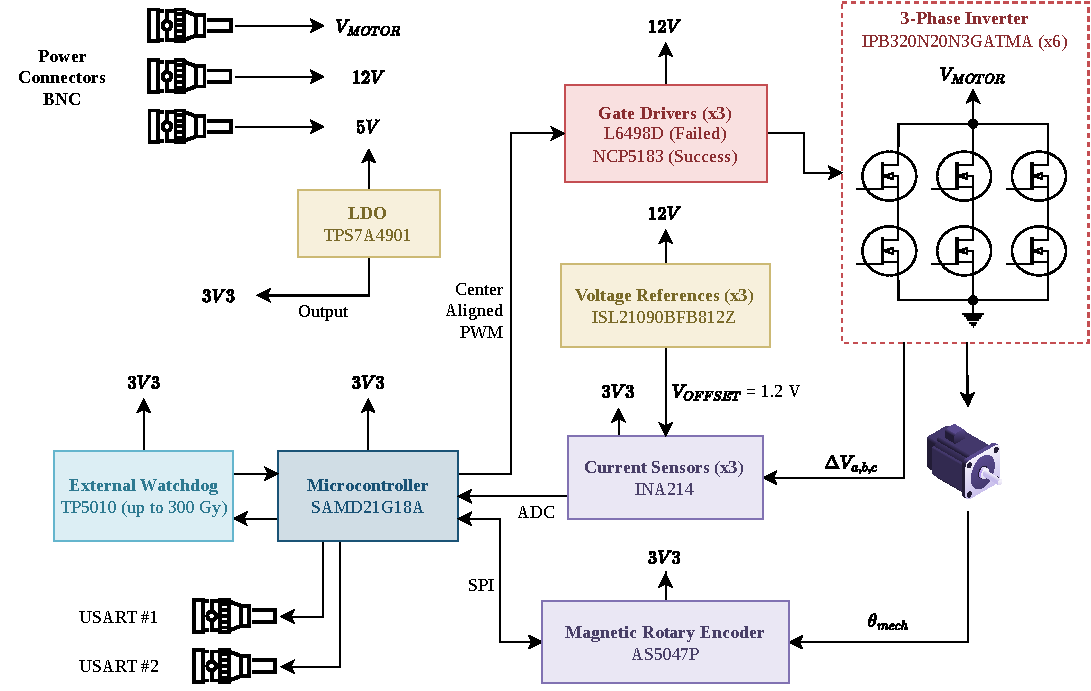
\includegraphics[width=\textwidth,keepaspectratio]{04_DesignForRadiationEnvironment/images/SecondIterationSystem.pdf}
  \caption{Σχηματική απεικόνιση υψηλού επιπέδου του τελικού συστήματος και των κρίσιμων διασυνδέσεών του.}
  \label{fig:final-pcb-system-architecture-gr}
\end{figure}

\begin{figure}[H]
  \centering
  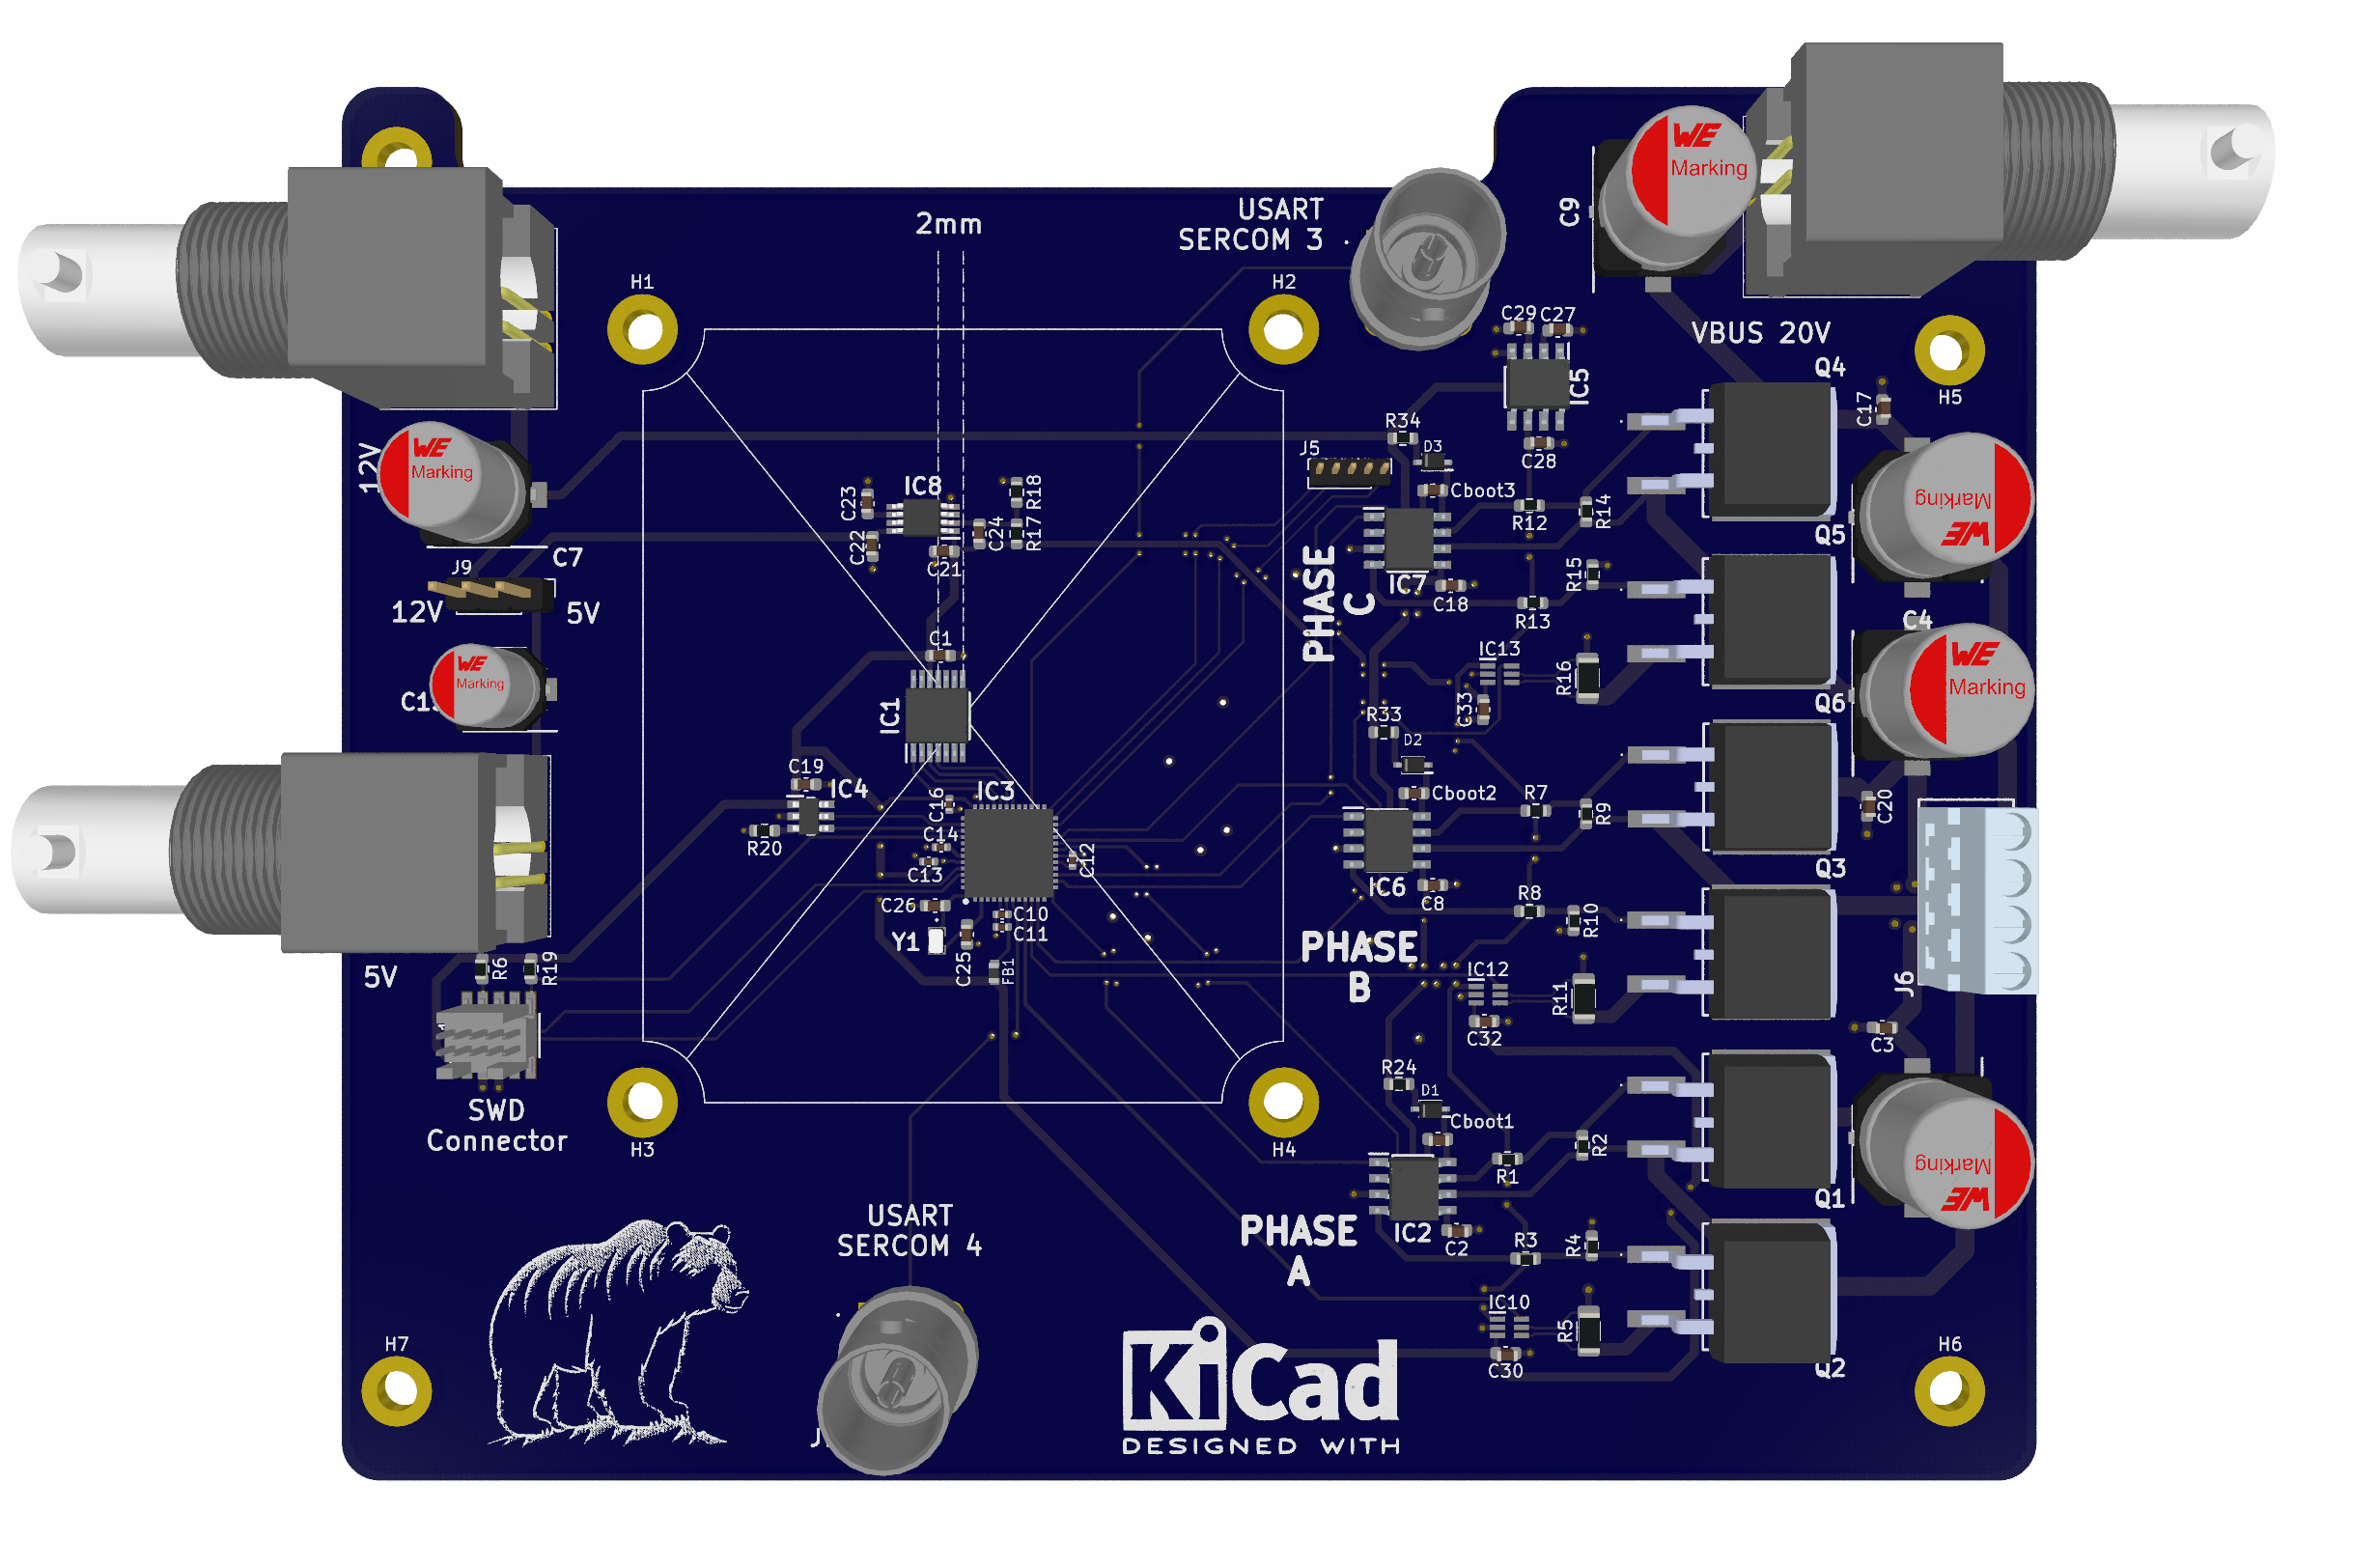
\includegraphics[width=0.75\textwidth,keepaspectratio]{04_DesignForRadiationEnvironment/images/BLDC_Motor_Driver.png}
  \caption{Τρισδιάστατη απεικόνιση της τελικής πλακέτας, παραγόμενη με το ενσωματωμένο εργαλείο φωτορεαλιστικής απεικόνισης του KiCad~9.0.}
  \label{fig:final-pcb-3d-render-gr}
\end{figure}

Στη συνέχεια, ένα από τα σημαντικότερα στάδια είναι ο σχεδιασμός των δοκιμών υπό ακτινοβολία~(radiation tests), τόσο σε επίπεδο διαδικασίας όσο και σε κατασκευαστικό επίπεδο. Ο πρωταρχικός στόχος της πειραματικής διάταξης~(test setup) είναι η μέγιστη παρατηρησιμότητα του συστήματος, καθώς και η διατήρηση της μηχανικής του ακεραιότητας. Η μηχανολογική διάταξη έχει ως στόχο να στερεώσει τον κινητήρα επάνω από το PCB, στην κατάλληλη θέση και απόσταση, ώστε ο μόνιμος μαγνήτης που χρησιμοποιείται από τον encoder να είναι όσο το δυνατόν πιο κεντραρισμένος και σε απόσταση περίπου ενός χιλιοστού από το ολοκληρωμένο κύκλωμα. Επίσης, ένας resolver τοποθετείται κεντραρισμένα και ομοαξονικά με τον ρότορα και προσφέρει μία ανεξάρτητη αναφορά της γωνιακής θέσης. Η αναφορά αυτή χρησιμοποιείται στη συνέχεια για την αξιολόγηση της απόδοσης του συστήματος, αλλά και κατά τη διάρκεια των δοκιμών για την αναγνώριση και αποκατάσταση περιόδων δυσλειτουργίας.

Οι δοκιμές υπό ακτινοβολία πραγματοποιήθηκαν σε τρεις διαφορετικές εγκαταστάσεις, καθεμία από τις οποίες χαρακτηρίζεται από διαφορετικό περιβάλλον και είδος ακτινοβολίας. Αρχικά, ο μαγνητικός encoder δοκιμάστηκε στο Paul Scherrer Institute~(PSI) και, πιο συγκεκριμένα, στο Proton Irradiation Facility~(PIF). Στην εγκατάσταση αυτή χρησιμοποιείται δέσμη πρωτονίων ενέργειας 200~MeV, με πολύ υψηλούς ρυθμούς ιονίζουσας δόσης. Υπό αυτό το περιβάλλον, το σύστημα μπορεί να υποβαθμιστεί λόγω Συνολικής Ιονίζουσας Δόσης~(TID) και Βλάβης Εκτόπισης~(Displacement Damage), καθώς και να παρουσιάσει Single Event Effects~(SEE). Η δοκιμή πραγματοποιήθηκε έως TID 1~kGy και τα αποτελέσματα έδειξαν ότι ο encoder αποτελεί κατάλληλη επιλογή για το πρωτότυπο, καθώς δεν παρουσίασε σημάδια μόνιμης υποβάθμισης, παρότι παρατηρήθηκαν παροδικά συμβάντα που αποδόθηκαν σε SEE.

Οι δοκιμές σε επίπεδο πλήρους συστήματος πραγματοποιήθηκαν στις εγκαταστάσεις CC60, όπου το σύστημα ακτινοβολείται με ακτίνες γάμμα από πηγή κοβαλτίου-60 και συνεπώς αξιολογείται κυρίως ως προς τη συσσωρευμένη TID, καθώς και στο CHARM. Το CHARM είναι μία εγκατάσταση μικτού πεδίου, στην οποία δέσμη πρωτονίων ορμής 24~GeV/$c$ εξάγεται από το Proton Synchrotron και προσπίπτει σε στόχο. Ανάλογα με το υλικό του στόχου, παράγεται ένα σύνθετο φάσμα δευτερογενών σωματιδίων, με ενέργειες που εκτείνονται από την κλίμακα των MeV έως εκείνη των GeV. Επομένως, το περιβάλλον αυτό είναι περισσότερο αντιπροσωπευτικό των πεδίων ακτινοβολίας που συναντώνται στις εγκαταστάσεις επιταχυντών του CERN. Στην παρούσα εργασία, τα κύρια αποτελέσματα αφορούν την αξιολόγηση της επαναληψιμότητας του σερβοκινητήριου συστήματος υπό ακτινοβολία γάμμα, ενώ συμπληρωματικά παρουσιάζονται και αποτελέσματα από τις δοκιμές στο CHARM.

Σε όλες τις δοκιμές που αναφέρονται παρακάτω, ο MCU προγραμματίστηκε ώστε περίπου κάθε 15~s να διατάζει τον ρότορα να μετακινηθεί σε διαφορετική θέση. Πιο συγκεκριμένα, ορίζονται τέσσερις διαφορετικές γωνίες, οι οποίες διατάσσονται κυκλικά και διαδοχικά. Η επαναληψιμότητα του συστήματος ορίζεται ως η ικανότητα του ρότορα να επιστρέφει κάθε φορά στην ίδια θέση. Εφόσον ορίστηκαν τέσσερις διαφορετικές γωνίες, καθεμία εξετάζεται μεμονωμένα και, επιπλέον, υπολογίζεται μία συγκεντρωτική~(pooled) μετρική τυπικής απόκλισης για το σύνολο των θέσεων.

Κατά την πρώτη δοκιμή στην εγκατάσταση CC60, το σύστημα εμφάνισε σταθερή απόδοση όσον αφορά την ποιότητα του ελέγχου και την επαναληψιμότητα. Παρ' όλα αυτά, έπαψε να λειτουργεί ομαλά μετά από TID περίπου 312.5~Gy. Έπειτα από ενδελεχή έλεγχο μετά την ακτινοβόληση, προέκυψε ότι και τα τρία κυκλώματα οδήγησης πυλών L6498D είχαν καταστεί μη λειτουργικά. Παράλληλα, στη γραμμή τροφοδοσίας τους παρατηρήθηκε προοδευτική αύξηση της κατανάλωσης, η οποία στο τέλος της ακτινοβόλησης έφθασε περίπου το 740~\% σε σχέση με την αρχική τιμή.

Με την αντικατάσταση των gate drivers από τα NCP5183, η δοκιμή επαναλήφθηκε και το σύστημα παρέμεινε πλήρως λειτουργικό έως συνολική TID περίπου 646.8~Gy, υπερβαίνοντας τον αρχικό στόχο των 500~Gy. Μετά το σημείο αυτό εμφανίστηκαν έντονος θόρυβος, ταλαντώσεις και ακανόνιστη κίνηση του ρότορα, πριν το σύστημα εισέλθει σε κατάσταση πλήρους αστοχίας. Ωστόσο, έως το τελευταίο πλήρως λειτουργικό παράθυρο δόσης δεν παρατηρήθηκε μετρήσιμη υποβάθμιση της επαναληψιμότητας. Η συγκεντρωτική επαναληψιμότητα $3\sigma$ παρέμεινε σχεδόν σταθερή μεταξύ $0.33^{\circ}$ και $0.39^{\circ}$, χωρίς εμφανή αυξητική ή μειωτική τάση έως το τελευταίο παράθυρο στα 626.3~Gy. Η Θέση~2 εμφάνισε τη μεγαλύτερη τοπική διασπορά, με μέγιστη τιμή $0.4738^{\circ}$, ενώ η Θέση~3 την καλύτερη επίδοση, με ελάχιστη τιμή $0.2630^{\circ}$. Η εξέλιξη της τοπικής και της συγκεντρωτικής επαναληψιμότητας $3\sigma$ ως συνάρτηση της συσσωρευμένης TID παρουσιάζεται στην εικόνα~\ref{fig:ncp5183-3s-gr}. Οι διαφορές μεταξύ των επιμέρους γωνιών αποδίδονται κυρίως σε μηχανολογικές ατέλειες που σχετίζονται με την ευθυγράμμιση και την απόσταση του μαγνήτη από το ολοκληρωμένο κύκλωμα του encoder, καθώς δεν παρατηρείται κάποια συστηματική τάση που να μπορεί να αποδοθεί στην ακτινοβολία.

\begin{figure}[H]
    \centering
    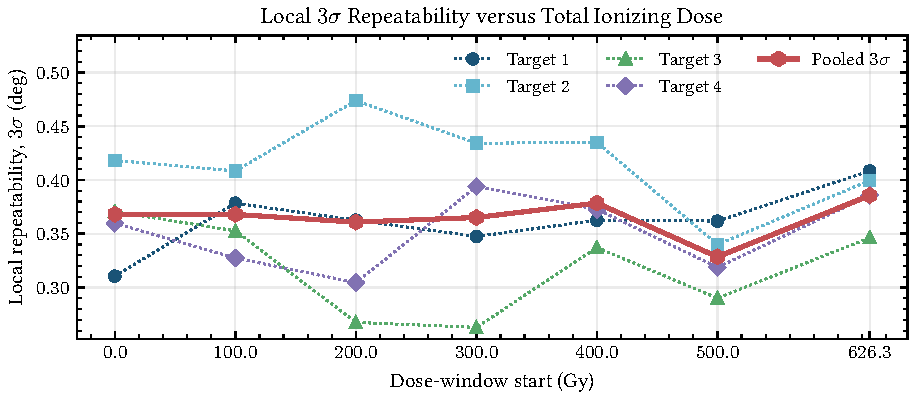
\includegraphics[width=\textwidth,keepaspectratio]{06_RadiationTestsResults/images-ncp5183/three_sigma.pdf}
    \caption{Τοπική επαναληψιμότητα τοποθέτησης $3\sigma$ και συγκεντρωτική τιμή αναφοράς του συστήματος ως συνάρτηση της συσσωρευμένης συνολικής ιονίζουσας δόσης.}
    \label{fig:ncp5183-3s-gr}
\end{figure}

Συμπληρωματικά προς τις παραπάνω δοκιμές, πραγματοποιήθηκαν και δοκιμές στο CHARM. Αν και χρονικά προηγήθηκαν των δοκιμών στο CC60 και χρησιμοποιούσαν τα L6498D, αξιοποιούνται για την εξαγωγή συμπερασμάτων σχετικά με τα SEE και την αποτελεσματικότητα τεχνικών μετριασμού σφαλμάτων. Στην εικόνα~\ref{fig:charm-cross-sections-gr} παρουσιάζεται η σύγκριση των ενεργών διατομών~(cross-sections) για δύο διαφορετικές κατηγορίες συμβάντων. Η πρώτη κατηγορία αφορά την απότομη διακοπή της λειτουργίας του MCU, η οποία απαιτούσε επανεκκίνηση για την αποκατάστασή του και ταξινομήθηκε ως Single Event Functional Interrupt~(SEFI). Ως ξεχωριστή κατηγορία ταξινομήθηκαν οι περιπτώσεις κατά τις οποίες ο MCU συνέχιζε να λειτουργεί, αλλά είχε χαθεί η ελεγξιμότητα του συστήματος, με συμπτώματα όπως ανεξέλεγκτη κίνηση ή ακινητοποίηση του ρότορα. Τα συμβάντα αυτά ονομάστηκαν Control Corruption και μπορούν, μεταξύ άλλων, να προκληθούν από αντιστροφή bit που αλλοιώνει κρίσιμες παραμέτρους του αλγορίθμου, οι οποίες υπολογίζονται κατά την εκκίνηση και αποθηκεύονται στη RAM.

Η ευαισθησία του MCU σε SEFI εξαρτάται κυρίως από την εσωτερική αρχιτεκτονική του και δεν μπορεί να μειωθεί άμεσα μέσω της συγκεκριμένης τεχνικής λογισμικού, αν και η λειτουργία του συστήματος μπορεί να αποκατασταθεί μέσω μηχανισμών επιτήρησης και επανεκκίνησης. Για την αντιμετώπιση των συμβάντων Control Corruption εφαρμόστηκε δοκιμαστικά η τεχνική Triple Modular Redundancy~(TMR). Σε επίπεδο λογισμικού, οι κρίσιμες μεταβλητές αποθηκεύονται σε τρία διαφορετικά σημεία της μνήμης, σε επαρκή απόσταση μεταξύ τους, ώστε να μειώνεται η πιθανότητα περισσότερα από ένα αντίγραφα να επηρεαστούν από το ίδιο SEE. Κατά τη χρήση τους από τον αλγόριθμο διαβάζονται και τα τρία αντίγραφα και επιλέγεται η τιμή της πλειοψηφίας. Εάν ένα αντίγραφο διαφέρει, διορθώνεται με αντικατάστασή του από την πλειοψηφική τιμή.

Η ενεργός διατομή ενός τύπου συμβάντος υπολογίζεται ως ο αριθμός των καταγεγραμμένων συμβάντων διαιρεμένος με τη συνολική fluence των σωματιδίων υψηλής ενέργειας~(HEH), ενώ τα άνω όρια αβεβαιότητας υπολογίζονται με βάση στατιστική Poisson για διάστημα εμπιστοσύνης 95~\%. Στην πρώτη καμπάνια, χωρίς ενεργοποιημένη την τεχνική TMR, καταγράφηκαν 38 συμβάντα MCU SEFI και 21 συμβάντα Control Corruption για fluence $3.06\times10^{11}$~cm$^{-2}$. Οι αντίστοιχες ενεργές διατομές ήταν $1.24\times10^{-10}$~cm$^{2}$ και $6.86\times10^{-11}$~cm$^{2}$. Στη δεύτερη καμπάνια, με ενεργοποιημένη την TMR, καταγράφηκαν 28 συμβάντα MCU SEFI και 11 συμβάντα Control Corruption για παρόμοια fluence, $3.05\times10^{11}$~cm$^{-2}$, με ενεργές διατομές $9.19\times10^{-11}$~cm$^{2}$ και $3.61\times10^{-11}$~cm$^{2}$, αντίστοιχα. Οι ενεργές διατομές των MCU SEFI είναι στατιστικά συμβατές μεταξύ των δύο δοκιμών. Αντίθετα, η ενεργός διατομή των συμβάντων Control Corruption μειώθηκε κατά περίπου 47~\% με την εφαρμογή της TMR, γεγονός που υποδεικνύει ότι η τεχνική ήταν αποτελεσματική στον περιορισμό της διάδοσης σφαλμάτων προς την απώλεια ελεγξιμότητας του κινητήρα.

\begin{figure}[H]
    \centering
    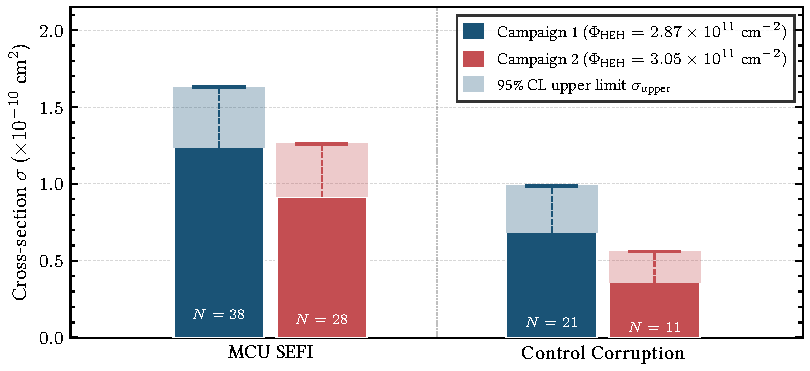
\includegraphics[width=0.9\textwidth,keepaspectratio]{06_RadiationTestsResults/charm-plots/cross_sections_charm.pdf}
    \caption{Σύγκριση των ενεργών διατομών SEE μεταξύ των δύο καμπανιών ακτινοβόλησης στο CHARM. Οι ενεργές διατομές των MCU SEFI είναι στατιστικά συμβατές, ενώ η ενεργός διατομή των συμβάντων Control Corruption μειώνεται στη δεύτερη καμπάνια, κατά την οποία ήταν ενεργή η τεχνική μετριασμού σφαλμάτων μέσω λογισμικού.}
    \label{fig:charm-cross-sections-gr}
\end{figure}

Η προτεινόμενη διάταξη πέτυχε πολύ υψηλή αντοχή ως προς την TID, αλλά η τελική έκδοση με τα NCP5183 δεν αξιολογήθηκε στην εγκατάσταση CHARM, όπου θα μπορούσε να παρουσιάσει επιπλέον υποβάθμιση λόγω Displacement Damage και SEE. Επομένως, η δοκιμή της στο CHARM αποτελεί το επόμενο λογικό βήμα. Στη συνέχεια, θα πρέπει να δοθεί σαφέστερη κατεύθυνση ως προς την τελική εφαρμογή του συστήματος. Ο συγκεκριμένος MCU, ως Cortex-M0+, διαθέτει περιορισμένους υπολογιστικούς πόρους για έλεγχο κινητήρα υψηλότερου επιπέδου και πολυπλοκότητας. Για τον λόγο αυτό, θα μπορούσε να εξεταστεί η μετάβαση σε άλλη πλατφόρμα, όπως ισχυρότερος MCU ή FPGA.

\end{greek}
